% 1. SOLUCIÓN Y RESULTADOS
\vspace{0.8em}
\noindent
{\renewcommand{\arraystretch}{1.0}
\begin{tabularx}{\linewidth}{|>{\centering\arraybackslash}X|}
    \hline
    \rowcolor{tablebackground}
    \textbf{\large\color{white} SOLUCIÓN Y RESULTADOS} \\
\end{tabularx}
}

\vspace{-1.5em}
\subsection{EJERCICIOS/PROBLEMAS PROPUESTOS}

\noindent\textbf{\color{mauve} Contexto del Caso de Estudio: Editorial QSY}\par
\noindent El presente desarrollo aborda la planificación ágil para el sistema de gestión comercial y control de existencias de la empresa editorial \textbf{QSY} (Arequipa), dedicada a la producción y comercialización de material bibliográfico educativo y médico en lengua quechua (catálogo base de 10 publicaciones). La empresa distribuye sus libros exclusivamente a través de tres distribuidoras aliadas presenciales (Trilce, Siglo XX y Jerusalén) en la ciudad de Arequipa. La problemática crítica levantada en la fase de ingeniería de requisitos evidenció que dos de los tres locales carecen de internet fijo por cable (los distribuidores utilizan planes de datos móviles propios de señal intermitente), registran ventas en cuadernos manuales, manejan boletas físicas de talonario y sufren demoras de más de una hora diaria en el cuadre manual de liquidaciones. Para dar solución definitiva a esta situación, se diseñó una solución basada en una \textbf{aplicación web responsiva (Mobile-First SPA)} con persistencia local en \texttt{IndexedDB} para operación tolerante a fallos de conexión (modo offline), respaldada por una API REST centralizada y base de datos relacional con aislamiento multi-sucursal mediante RBAC.

\vspace{1em}
\noindent\textbf{\large PARTE 1: PRODUCT BACKLOG}

\subsubsection*{\color{mauve} 1. Definición de Requerimientos y Estructura del Backlog}
\noindent Se identificaron y formularon \textbf{18 requerimientos funcionales} transformados rigurosamente en Historias de Usuario bajo el estándar ágil (\textit{Como [rol], quiero [acción], para [beneficio esperado]}). Los requerimientos se agrupan en cinco módulos funcionales que cubren la totalidad del ciclo de valor de la editorial:
\begin{enumerate}
    \item \textbf{Módulo 1: Distribución y Administración de Sedes (HU-01 a HU-06):} Gestión de perfiles RBAC, alta de distribuidoras aliadas, catálogo centralizado con precios y comisiones fijas inmutables, control de despachos en consignación y monitoreo de existencias.
    \item \textbf{Módulo 2: Registro de Ventas y Comprobantes en Sucursal (HU-07 a HU-11):} Venta táctil optimizada para celular en mostrador ($< 2$ minutos), almacenamiento local en \texttt{IndexedDB} con sincronización diferida ante cortes de red, emisión de ticket de venta interno en formato PDF, captura obligatoria de DNI/nombres del alumno y monitor de inventario local.
    \item \textbf{Módulo 3: Reabastecimiento e Inventario Central (HU-12 a HU-14):} Solicitud digital de pedidos de reposición desde la web, aprobación/despacho desde almacén central y registro de ingresos de imprenta.
    \item \textbf{Módulo 4: Liquidación Diaria de Ventas y Comisiones (HU-15 a HU-17):} Generación de balance de liquidación diario automatizado (reducción de 1 hora a 10 segundos), arqueo y conciliación de saldos en efectivo físico (con regularización directa por el distribuidor de pagos recibidos vía billeteras digitales personales) y pago consolidado de comisiones fijas a los distribuidores.
    \item \textbf{Módulo 5: Trazabilidad, Auditoría y Reportes Gerenciales (HU-18 a HU-19):} Búsqueda y validación de reclamos de garantía mediante DNI de alumno y panel analítico gerencial consolidado.
\end{enumerate}

\subsubsection*{\color{mauve} 2. Tabla Integral del Product Backlog}
\noindent En la Tabla~\ref{tab:product_backlog} se consolida el Product Backlog completo del proyecto, priorizado según la técnica MoSCoW (\textit{Must Have}, \textit{Should Have}, \textit{Could Have}) y estimado en (\textit{Story Points} - SP):

\begin{xltabular}{\textwidth}{|c|X|c|c|c|}
\caption{Product Backlog Consolidado de la Editorial QSY} \label{tab:product_backlog} \\
\hline
\rowcolor{graya}
\textbf{ID} & \textbf{Narrativa Ágil (Descripción de la Historia de Usuario)} & \textbf{Prioridad} & \textbf{SP} & \textbf{Release} \\
\hline
\endfirsthead
\hline
\rowcolor{graya}
\textbf{ID} & \textbf{Narrativa Ágil (Descripción de la Historia de Usuario)} & \textbf{Prioridad} & \textbf{SP} & \textbf{Release} \\
\hline
\endhead
\hline
\multicolumn{5}{|r|}{\textit{Continúa en la siguiente página\dots}} \\
\hline
\endfoot
\hline
\endlastfoot
\textbf{HU-01} & \textbf{Como} Administrador, \textbf{quiero} autenticar usuarios con roles (Admin, Logística, Distribuidor) y restringir permisos por sede, \textbf{para} asegurar aislamiento total entre locales. & Must Have & 8 & Sprint 1 \\
\hline
\textbf{HU-02} & \textbf{Como} Administrador, \textbf{quiero} registrar y administrar los puntos de venta distribuidores, \textbf{para} mantener el padrón oficial y habilitar la asignación de usuarios y stock. & Must Have & 5 & Sprint 1 \\
\hline
\textbf{HU-03} & \textbf{Como} Administrador, \textbf{quiero} gestionar el catálogo de publicaciones y fijar precios y comisiones unitarias, \textbf{para} garantizar tarifas uniformes e inmutables en ventanilla. & Must Have & 5 & Sprint 1 \\
\hline
\textbf{HU-04} & \textbf{Como} Encargado de Logística, \textbf{quiero} registrar despachos en consignación a cada distribuidora, \textbf{para} transferir existencias formales desde el almacén central. & Must Have & 5 & Sprint 2 \\
\hline
\textbf{HU-05} & \textbf{Como} Distribuidor, \textbf{quiero} confirmar la recepción física de libros consignados, \textbf{para} validar el stock disponible en mostrador y reportar discrepancias. & Must Have & 3 & Sprint 2 \\
\hline
\textbf{HU-06} & \textbf{Como} Encargado de Logística, \textbf{quiero} consultar existencias por sede y en consolidado global, \textbf{para} conocer la disponibilidad real de libros en toda la red. & Must Have & 5 & Sprint 2 \\
\hline
\textbf{HU-07} & \textbf{Como} Distribuidor, \textbf{quiero} registrar ventas presenciales ágiles desde mi celular, \textbf{para} completar la atención en ventanilla en menos de 2 minutos. & Must Have & 8 & Sprint 3 \\
\hline
\textbf{HU-08} & \textbf{Como} Distribuidor, \textbf{quiero} registrar ventas en modo offline mediante IndexedDB, \textbf{para} operar sin interrupciones ante fallas de cobertura de datos móviles. & Must Have & 8 & Sprint 3 \\
\hline
\textbf{HU-09} & \textbf{Como} Distribuidor, \textbf{quiero} generar un ticket de venta interno en PDF (enviar por WhatsApp o imprimir), \textbf{para} entregar comprobante de respaldo al estudiante. & Must Have & 5 & Sprint 3 \\
\hline
\textbf{HU-10} & \textbf{Como} Distribuidor, \textbf{quiero} registrar DNI, nombre del alumno y método de pago (Efectivo/Yape), \textbf{para} garantizar trazabilidad operativa de la transacción. & Must Have & 3 & Sprint 3 \\
\hline
\textbf{HU-11} & \textbf{Como} Distribuidor, \textbf{quiero} visualizar el inventario remanente de mi propio local, \textbf{para} controlar el balance físico diario sin exponer cifras de otras sedes. & Must Have & 5 & Sprint 4 \\
\hline
\textbf{HU-12} & \textbf{Como} Distribuidor, \textbf{quiero} emitir solicitudes web de reposición de stock hacia Logística, \textbf{para} evitar quiebres de inventario sin depender de llamadas telefónicas. & Must Have & 4 & Sprint 4 \\
\hline
\textbf{HU-13} & \textbf{Como} Encargado de Logística, \textbf{quiero} procesar pedidos de reposición pendientes, \textbf{para} autorizar y despachar nuevos lotes según disponibilidad central. & Must Have & 5 & Sprint 4 \\
\hline
\textbf{HU-14} & \textbf{Como} Encargado de Logística, \textbf{quiero} registrar entradas por lotes de imprenta, \textbf{para} actualizar el inventario primario y costos de fabricación. & Should Have & 5 & Sprint 4 \\
\hline
\textbf{HU-15} & \textbf{Como} Distribuidor, \textbf{quiero} generar el balance de liquidación diario automático en pantalla, \textbf{para} conciliar ventas, efectivo y transferencias en segundos. & Must Have & 8 & Sprint 5 \\
\hline
\textbf{HU-16} & \textbf{Como} Administrador, \textbf{quiero} validar arqueos y registrar pagos de comisiones fijas, \textbf{para} liquidar los honorarios monetarios pactados por libro vendido. & Must Have & 5 & Sprint 5 \\
\hline
\textbf{HU-17} & \textbf{Como} Administrador, \textbf{quiero} registrar gastos operativos y compras de insumos, \textbf{para} deducir costos auxiliares del flujo de caja del negocio. & Should Have & 4 & Sprint 5 \\
\hline
\textbf{HU-18} & \textbf{Como} Sucursal Virtual, \textbf{quiero} consultar compras por DNI de estudiante, \textbf{para} resolver garantías de libros y verificar claves de acceso virtual. & Should Have & 4 & Sprint 5 \\
\hline
\textbf{HU-19} & \textbf{Como} Administrador, \textbf{quiero} visualizar paneles gerenciales de ingresos y rotación, \textbf{para} tomar decisiones de reimpresión basadas en demanda real. & Could Have & 6 & Sprint 5 \\
\hline
\multicolumn{3}{|r|}{\textbf{Total de Puntos de Historia del Product Backlog (93 SP)}} & \textbf{93} & \\
\end{xltabular}

\vspace{1em}
\noindent\textbf{\large PARTE 2: SPRINT BACKLOG}

\subsubsection*{\color{mauve}1. Definición del Sprint 1}
\noindent Se estableció un ciclo de iteración (\textit{Sprint}) con una duración fija de \textbf{2 semanas} (10 días laborables). A continuación se fundamenta la planificación cuantitativa y cualitativa del Sprint 1:
\begin{itemize}
    \item \textbf{Objetivo del Sprint (\textit{Sprint Goal}):} ``Establecer los cimientos arquitectónicos del proyecto, el modelo de datos relacional y el sistema de control de acceso basado en roles (RBAC), permitiendo al Administrador registrar los puntos de venta distribuidores y configurar el catálogo oficial de publicaciones con sus precios y comisiones fijas inmutables''.
    \item \textbf{Capacidad del Equipo (\textit{Team Capacity}):} El equipo está integrado por 4 ingenieros. Considerando una dedicación académica a tiempo parcial de 15 horas semanales por persona, se obtiene una capacidad teórica de 120 horas-hombre para las dos semanas. Aplicando un factor de foco del 80\% ($0.80$) para absorber reuniones de sincronización ágil e imprevistos de integración, la \textbf{capacidad efectiva neta disponible es de 96 horas-hombre}.
    \item \textbf{Carga Asignada:} Para este primer sprint se comprometieron \textbf{18 Story Points}, traducidos en \textbf{54 horas-hombre de trabajo técnico directo}. Esto otorga un margen de holgura del 44\% (42 horas de reserva), mitigando riesgos derivados del montaje del entorno base y configuración de la infraestructura inicial.
\end{itemize}

\subsubsection*{\color{mauve}2. Selección de Requerimientos del Backlog}
\noindent Del Product Backlog se seleccionaron las siguientes tres historias prioritarias para el Sprint 1:
\begin{enumerate}
    \item \textbf{HU-01 (Autenticación y RBAC con aislamiento por sede - 8 SP):} Requisito angular de seguridad que previene la fuga de información comercial entre distribuidoras rivales.
    \item \textbf{HU-02 (Gestión del padrón de distribuidoras - 5 SP):} Entidad organizativa fundamental requerida para asignar usuarios, inventarios y despachos futuros.
    \item \textbf{HU-03 (Catálogo de publicaciones, precios y comisiones fijas - 5 SP):} Regla de negocio crítica pactada con gerencia para garantizar que los precios al público y las comisiones unitarias en soles sean inmutables por los vendedores.
\end{enumerate}

\subsubsection*{\color{mauve}3. Descomposición en Actividades Técnicas y Trazabilidad de Dependencias}
\noindent Las historias seleccionadas fueron descompuestas en \textbf{14 tareas técnicas de ingeniería de software}. Para garantizar el orden riguroso y la no colisión de actividades, se estableció una \textbf{red de precedencia y dependencias técnicas}:

\begin{itemize}
    \item \textbf{Tareas Fundacionales Bloqueantes (Yourdyy - Scrum Master / Arquitecto):} Las tareas de arquitectura y persistencia (\texttt{TASK-01-01}, \texttt{TASK-01-02}, \texttt{TASK-02-01} y \texttt{TASK-03-01}) representaron el cuello de botella inicial crítico. Sin el repositorio estructurado ni los esquemas relacionales DDL (\texttt{users}, \texttt{roles}, \texttt{branches}, \texttt{products}), ningún desarrollador backend o frontend podía avanzar. \textbf{Al momento de sustentación del presente informe, estas 4 tareas han sido completadas exitosamente al 100\% (Estado: \texttt{done})}, liberando formalmente el bloqueo sobre el resto del equipo.
    \item \textbf{Tareas Desbloqueadas Activas (En Proceso - \texttt{in-progress}):} Con la base de datos y el scaffolding operativos, se activaron de inmediato aquellas tareas prioritarias que respetan el límite de trabajo en curso (WIP) y permiten la concurrencia:
    \begin{itemize}
        \item \textbf{Leonardo (Backend):} Toma \texttt{TASK-01-03} (\textit{API REST de autenticación y tokens JWT}), ya que cuenta con el script DDL de usuarios listo.
        \item \textbf{Miguel (Frontend):} Toma \texttt{TASK-01-05} (\textit{Interfaz web móvil de login}), maquetando las pantallas Mobile-First sobre la estructura base del cliente web.
        \item \textbf{Dolly (QA / Product Owner):} Toma \texttt{TASK-01-06} (\textit{Pruebas de integración de seguridad y control RBAC}), iniciando en paralelo la elaboración de las matrices de pruebas funcionales y suites de validación automatizada basadas en Gherkin.
    \end{itemize}
    \item \textbf{Tareas Pendientes en Espera (Por hacer - \texttt{todo}):} El resto de tareas técnicas (\texttt{TASK-01-04}, \texttt{TASK-02-02}, \texttt{TASK-02-03}, etc.) se mantienen justificadamente en estado \texttt{todo} porque presentan dependencias lógicas directas sobre las tareas que actualmente están en desarrollo (por ejemplo, el middleware RBAC \texttt{TASK-01-04} exige tener primero la API de login operativa; las interfaces de sucursales \texttt{TASK-02-03} esperan la integración de sesión de usuario). Esta disciplina previene la dispersión del equipo y respeta estrictamente las políticas Kanban.
    \item \textbf{Trazabilidad en los Archivos Markdown (\texttt{.md}):} Cada tarea técnica ubicada en \texttt{sprint-backlog/tasks/} incorpora en su metadato YAML la propiedad formal \texttt{dependencias: [...]}, enlazando de forma bidireccional los identificadores de las tareas bloqueantes (ej. \texttt{[[TASK-01-01]]}, \texttt{[[TASK-01-02]]}), lo cual permite generar grafos de precedencia automáticos y navegación contextual dentro de Obsidian.
\end{itemize}

\noindent En la Tabla~\ref{tab:sprint_backlog} se presenta el estado de ejecución y trazabilidad del Sprint Backlog:

\begin{xltabular}{\textwidth}{|c|c|X|c|c|c|c|}
\caption{Sprint Backlog Técnico del Sprint 1 (54 horas-hombre)} \label{tab:sprint_backlog} \\
\hline
\rowcolor{graya}
\textbf{ID Tarea} & \textbf{HU Padre} & \textbf{Descripción Técnica de la Actividad} & \textbf{Componente} & \textbf{Responsable} & \textbf{Horas} & \textbf{Estado} \\
\hline
\endfirsthead
\hline
\rowcolor{graya}
\textbf{ID Tarea} & \textbf{HU Padre} & \textbf{Descripción Técnica de la Actividad} & \textbf{Componente} & \textbf{Responsable} & \textbf{Horas} & \textbf{Estado} \\
\hline
\endhead
\hline
\multicolumn{7}{|r|}{\textit{Continúa en la siguiente página\dots}} \\
\hline
\endfoot
\hline
\endlastfoot
\textbf{TASK-01-01} & HU-01 & Registro de Arquitectura ADR-01 y scaffolding base del proyecto & Arquitectura & Yourdyy & 4 h & \textbf{done} \\
\hline
\textbf{TASK-01-02} & HU-01 & Registro ADR-02 y script DDL de esquemas de usuarios y roles & Base de Datos & Yourdyy & 4 h & \textbf{done} \\
\hline
\textbf{TASK-01-03} & HU-01 & Endpoints REST de inicio de sesión y emisión de JWT firmado & Backend & Leonardo & 6 h & \textbf{in-progress} \\
\hline
\textbf{TASK-01-04} & HU-01 & Middleware de autorización RBAC y aislamiento de datos por sede & Backend & Leonardo & 4 h & todo \\
\hline
\textbf{TASK-01-05} & HU-01 & Interfaz web móvil (Mobile-First) de login y gestión de sesión & Frontend & Miguel & 5 h & \textbf{in-progress} \\
\hline
\textbf{TASK-01-06} & HU-01 & Pruebas de integración de seguridad y control de acceso RBAC & QA / Pruebas & Dolly & 3 h & \textbf{in-progress} \\
\hline
\textbf{TASK-02-01} & HU-02 & Migración DDL de tabla \texttt{branches} y relaciones de integridad & Base de Datos & Yourdyy & 3 h & \textbf{done} \\
\hline
\textbf{TASK-02-02} & HU-02 & Endpoints CRUD para gestión de distribuidoras y encargados & Backend & Leonardo & 4 h & todo \\
\hline
\textbf{TASK-02-03} & HU-02 & Interfaz web responsiva para administración del padrón de sedes & Frontend & Miguel & 5 h & todo \\
\hline
\textbf{TASK-02-04} & HU-02 & Pruebas funcionales de registro de sucursales y validaciones & QA / Pruebas & Dolly & 2 h & todo \\
\hline
\textbf{TASK-03-01} & HU-03 & Migración DDL de tabla \texttt{products} y tarifas comisionales & Base de Datos & Yourdyy & 3 h & \textbf{done} \\
\hline
\textbf{TASK-03-02} & HU-03 & Endpoints REST de catálogo oficial y bloqueo de edición no admin & Backend & Leonardo & 4 h & todo \\
\hline
\textbf{TASK-03-03} & HU-03 & Interfaz web móvil de catálogo y configuración de tarifas fijas & Frontend & Miguel & 5 h & todo \\
\hline
\textbf{TASK-03-04} & HU-03 & Pruebas de inmutabilidad de precios y validación de comisiones & QA / Pruebas & Dolly & 2 h & todo \\
\hline
\multicolumn{5}{|r|}{\textbf{Total de Horas-Hombre del Sprint 1}} & \textbf{54 h} & \\
\end{xltabular}

\vspace{0.8em}
\noindent\textbf{Balance y Ejecución de Cargas por Rol en el Sprint 1:}
\begin{itemize}
    \item \textbf{Yourdyy (Scrum Master / Arquitecto de Software):} 14 horas concluidas al 100\% (\texttt{done}) en el scaffolding inicial, definición de registros ADRs y creación de los esquemas DDL relacionales (\texttt{users}, \texttt{roles}, \texttt{branches}, \texttt{products}).
    \item \textbf{Leonardo (Desarrollador Backend Full-Stack):} 18 horas asignadas, con 6 horas activas en desarrollo (\texttt{TASK-01-03} en \texttt{in-progress}) y 12 horas en espera secuencial (\texttt{todo}).
    \item \textbf{Miguel (Desarrollador Frontend Mobile):} 15 horas asignadas, con 5 horas en desarrollo activo (\texttt{TASK-01-05} en \texttt{in-progress}) y 10 horas en espera secuencial (\texttt{todo}).
    \item \textbf{Dolly (Product Owner / QA Tester):} 7 horas asignadas, con 3 horas activas en diseño de pruebas (\texttt{TASK-01-06} en \texttt{in-progress}) y 4 horas pendientes de ejecución funcional final (\texttt{todo}).
\end{itemize}

\vspace{0.8em}
\noindent\textbf{\large PARTE 3: PLANIFICACIÓN ÁGIL}

\subsubsection*{\color{mauve} 1. Metodología de Estimación de Tareas (Story Points)}
\noindent En el marco de la gestión ágil adoptada, se estableció una clara distinción epistemológica y práctica entre dos niveles de estimación:
\begin{itemize}
    \item \textbf{Nivel Estratégico (Historias de Usuario en Story Points):} Se utiliza la técnica de \textit{Planning Poker} con la secuencia de Fibonacci modificada ($1, 2, 3, 5, 8, 13$). El puntaje relativo no mide tiempo cronológico directo, sino una función tripartita compuesta por: (1) \textbf{Complejidad técnica del problema}, (2) \textbf{Volumen intrínseco de trabajo} y (3) \textbf{Nivel de riesgo e incertidumbre} (ej. la operación offline de HU-08 recibe 8 SP debido al riesgo inherente a la sincronización en segundo plano con \texttt{IndexedDB}).
    \item \textbf{Nivel Operativo (Tareas Técnicas en Horas de Ingeniería):} Durante el Sprint Planning, cada Historia se descompone en actividades concretas estimadas en horas-hombre directas. Esta granularidad fina (entre 2 y 6 horas) permite medir la velocidad real del equipo y realizar un seguimiento certero en las reuniones diarias (\textit{Daily Standup}).
\end{itemize}

\subsubsection*{\color{mauve} 2. Diseño del Tablero Kanban y Límites de Trabajo en Curso (WIP)}
\noindent Para la gestión visual del flujo se diseñó un tablero Kanban interactivo montado sobre el entorno de Obsidian mediante bases relacionales (\texttt{.base}). El flujo se organiza en cuatro columnas de estado secuenciales:
\begin{enumerate}
    \item \textbf{To Do (Por hacer):} Depósito de tareas planificadas para el Sprint 1 que cuentan con especificación aprobada y están listas para ejecución.
    \item \textbf{In Progress (En progreso):} Tareas que están siendo activamente codificadas o diseñadas por los desarrolladores asignados.
    \item \textbf{In Review (En revisión):} Tareas que han concluido el desarrollo y están sujetas a revisión de pares mediante \textit{Pull Request} y pruebas de aceptación conducidas por QA.
    \item \textbf{Done (Terminado):} Tareas que cumplen de forma estricta el \textit{Definition of Done} (DoD).
\end{enumerate}

\noindent\textbf{Políticas de Límites WIP (\textit{Work In Progress}):} Para prevenir la sobrecarga cognitiva y mitigar cuellos de botella, se definieron límites cuantitativos explícitos:
\begin{itemize}
    \item \textbf{Límite WIP en In Progress = 3 tareas en simultáneo:} Evita la dispersión de esfuerzos en el equipo de desarrollo, promoviendo el principio ágil fundamental: \textit{``Dejar de empezar y comenzar a terminar''}.
    \item \textbf{Límite WIP en In Review = 2 tareas en simultáneo:} Garantiza que el rol de QA y las revisiones de arquitectura no se conviertan en un punto de acumulación de deuda técnica.
\end{itemize}

\begin{figure}[H]
    \centering
    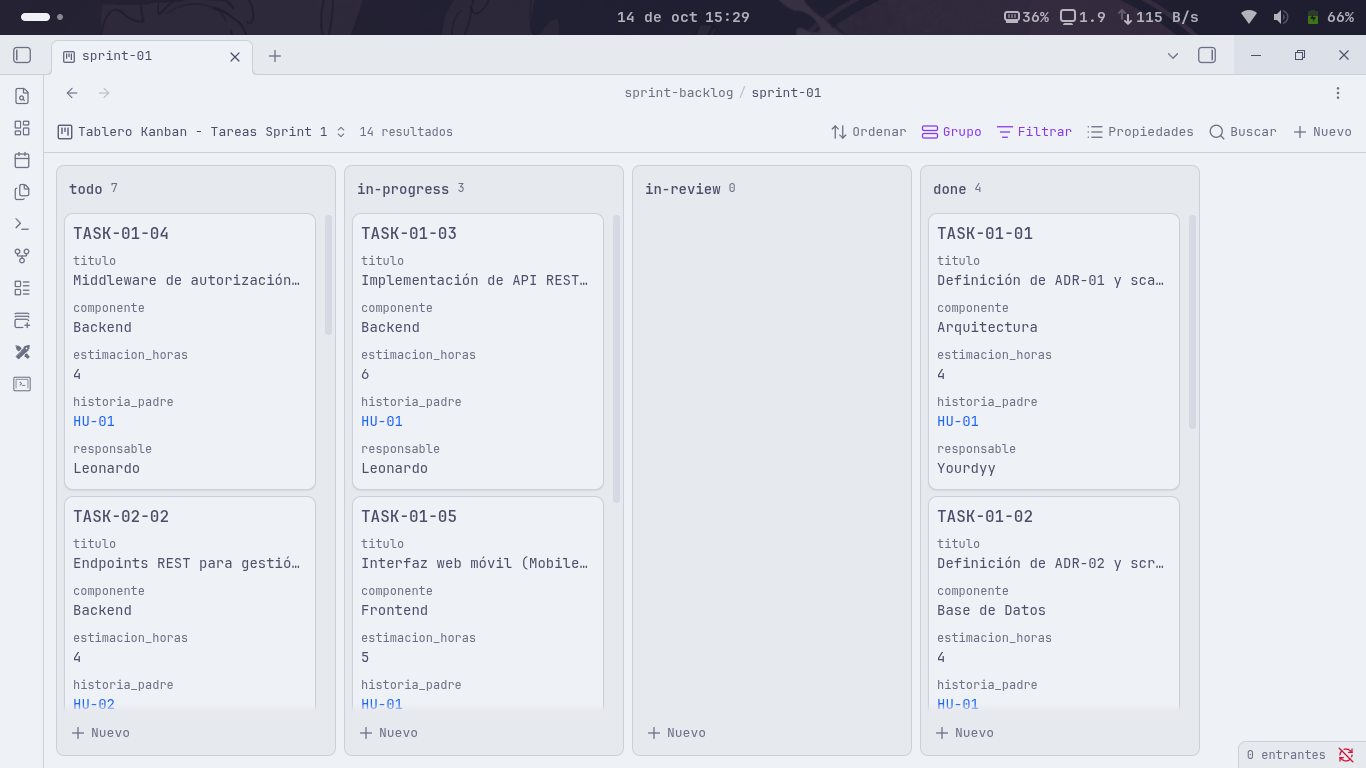
\includegraphics[width=0.92\linewidth]{img/imagen01.png}
    \caption{Tablero Kanban Interactivo del Sprint 1 en Obsidian (archivo \texttt{sprint-01.base})}
    \label{fig:kanban_sprint1}
\end{figure}

\subsubsection*{\color{mauve} 3. Definición del Flujo de Trabajo y Políticas de Calidad}
\noindent El flujo de trabajo ágil se rige por políticas explícitas de transición que garantizan la calidad del software antes y después de cada iteración:
\begin{itemize}
    \item \textbf{Definition of Ready (DoR - Criterio de Preparación):} Una Historia de Usuario solo puede ser seleccionada para un Sprint si cumple copulativamente: (1) Formato narrativo ágil estandarizado, (2) Criterios de aceptación detallados en lenguaje Gherkin (\textit{Given/When/Then}), (3) Dependencias arquitectónicas resueltas, (4) Estimación consensuada en Story Points y (5) Valor comercial validado por el Product Owner.
    \item \textbf{Definition of Done (DoD - Criterio de Terminación):} Una tarea o historia se declara finalizada únicamente cuando: (1) El código fuente está versionado en la rama correspondiente sin conflictos de Git, (2) Cumple los estándares de codificación y linter sin advertencias críticas, (3) Las pruebas unitarias e integración han sido ejecutadas satisfactoriamente por QA, (4) El Pull Request cuenta con aprobación técnica del Arquitecto (Yourdyy), y (5) Se encuentra desplegado y validado en entorno de pruebas local/staging.
\end{itemize}

\begin{figure}[H]
    \centering
    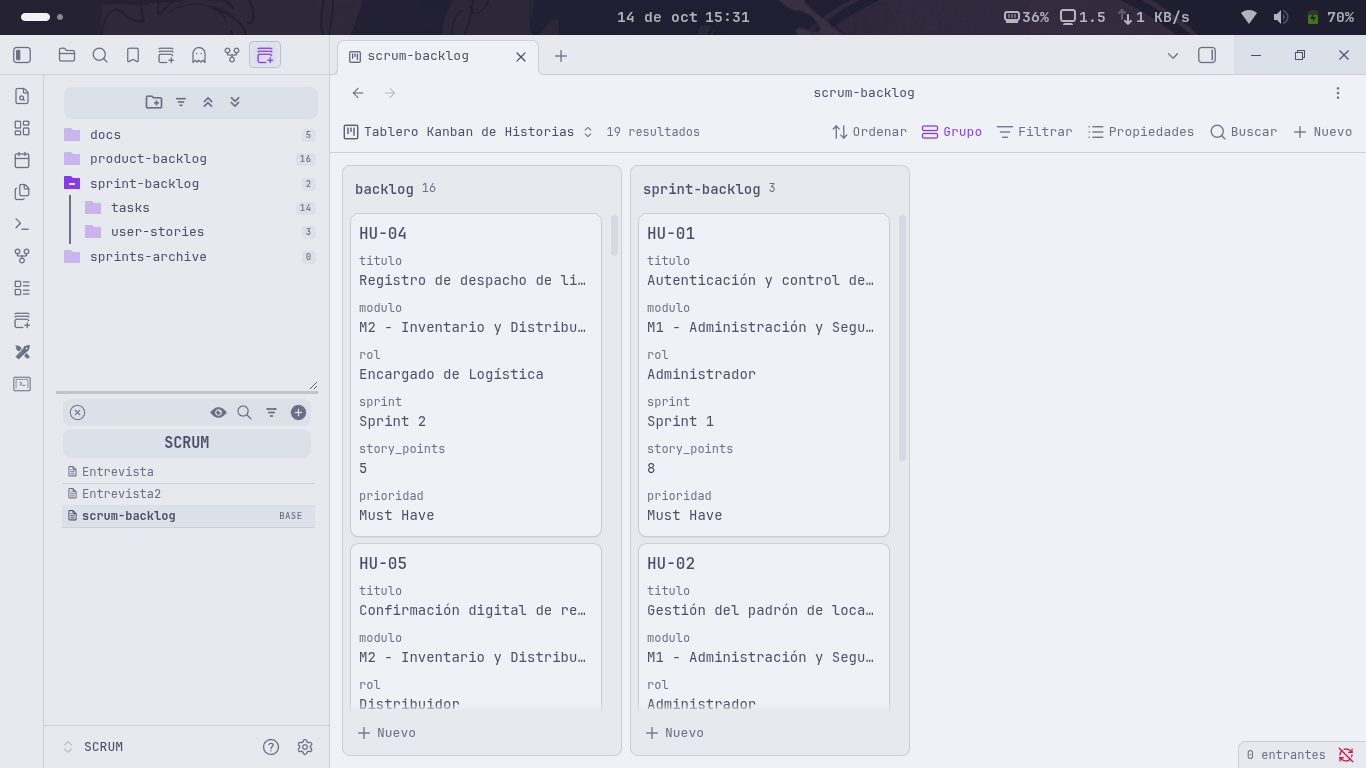
\includegraphics[width=0.92\linewidth]{img/imagen02.png}
    \caption{Product Backlog Consolidado y Estructura Relacional en Obsidian (archivo \texttt{scrum-backlog.base})}
    \label{fig:backlog_obsidian}
\end{figure}

\vspace{0.8em}
\noindent\textbf{\large PARTE 4: PRODUCTO MÍNIMO VIABLE (PMV)}

\subsubsection*{\color{mauve} 1. Identificación del Producto Mínimo Viable (PMV)}
\noindent El Producto Mínimo Viable (PMV) del proyecto editorial \textbf{QSY} abarca las \textbf{18 Historias de Usuario priorizadas (93 Story Points)}, distribuidas armónicamente a lo largo del roadmap de \textbf{5 Sprints de 2 semanas (10 semanas en total)}. Se determinó técnicamente que un PMV que prescindiera de alguno de los 5 módulos operativos resultaría disfuncional para el negocio:
\begin{itemize}
    \item La venta presencial no puede operar sin un catálogo oficial de precios fijos ni sin confirmación de despachos consignados.
    \item La operación en locales carentes de internet exige indispensablemente el mecanismo offline con \texttt{IndexedDB}.
    \item La sostenibilidad operativa de la red de librerías aliadas depende críticamente de la conciliación diaria automatizada de liquidaciones y del pago puntual de comisiones fijas en soles por cada título vendido.
\end{itemize}

\subsubsection*{\color{mauve} 2. Justificación Multidimensional de Viabilidad del PMV}
\noindent La viabilidad integral del PMV se fundamenta en cuatro dimensiones estratégicas de ingeniería de software y gestión empresarial:
\begin{enumerate}
    \item \textbf{Viabilidad Técnica:}
    \begin{itemize}
        \item \textit{Arquitectura Liviana y Desacoplada:} La solución se diseñó como una Single Page Application (SPA) responsiva con enfoque Mobile-First, eliminando los sobrecostos de licenciamiento y desarrollo multiplataforma nativo (Android/iOS).
        \item \textit{Resiliencia ante Desconexión:} La integración de \texttt{IndexedDB} permite encolar ventas transaccionales localmente en el navegador del celular del vendedor y sincronizarlas automáticamente con el servidor central al restablecerse la cobertura móvil, solucionando la precariedad de infraestructura de telecomunicaciones en 2 de las 3 sucursales.
        \item \textit{Aislamiento y Escalabilidad Relacional:} El modelo relacional en PostgreSQL garantiza la estricta partición lógica de registros entre distribuidoras, garantizando tiempos de respuesta menores a 2 segundos en consultas operativas.
    \end{itemize}
    \item \textbf{Viabilidad Operativa:}
    \begin{itemize}
        \item \textit{Facilidad de Uso y Curva de Adopción Rápida:} Las interfaces móviles están concebidas para operadores no técnicos, reduciendo el proceso de venta presencial a un flujo intuitivo de 3 toques que insume menos de 2 minutos por transacción.
        \item \textit{Erradicación de Fricciones Contables:} El proceso de liquidación diaria, que históricamente demandaba más de 1 hora de revisión de cuadernos físicos y conteo de boletas en papel, se automatiza a un balance digital instantáneo generado en menos de 10 segundos, eliminando discrepancias entre vendedores y la administración.
    \end{itemize}
    \item \textbf{Viabilidad Económica:}
    \begin{itemize}
        \item \textit{Aprovechamiento de Infraestructura Existente:} El sistema no requiere inversiones inmediatas en nuevo hardware ni en servicios cloud de alta tarificación, dado que se desplegará sobre el servidor VPS de Hostinger (2 vCPU, 8 GB RAM) actualmente subutilizado por la editorial.
        \item \textit{Estructura Presupuestal Sostenible:} El costo total estimado del proyecto asciende a S/ 31,500.00 (cubriendo 1,150 horas-hombre de desarrollo, aseguramiento de la calidad y contingencias), monto recuperable a corto plazo gracias al corte drástico de mermas de inventario y erradicación de errores humanos en la recaudación diaria.
    \end{itemize}
    \item \textbf{Viabilidad de Negocio y Estratégica:}
    \begin{itemize}
        \item \textit{Cumplimiento de Reglas de Negocio Centrales:} Garantiza la inmutabilidad de los precios de venta fijados por gerencia y el cómputo automático de las comisiones fijas pactadas con los distribuidores, evitando ventas discrecionales no autorizadas.
        \item \textit{Trazabilidad Total para Reclamos y Soporte:} La captura sistemática del DNI y nombres del estudiante comprador permite resolver reclamos de garantía y otorgar credenciales a recursos educativos digitales en segundos, elevando la reputación de marca de la editorial en el mercado educativo quechua.
    \end{itemize}
\end{enumerate}

\hrule
\vspace{0.8em}

\subsection{CUESTIONARIO}

\noindent\textbf{\color{mauve} 1. ¿Qué es Scrum y cuáles son sus componentes?}\par
\noindent Scrum es un marco de trabajo adaptativo, iterativo e incremental basado en el empirismo (transparencia, inspección y adaptación) y el pensamiento \textit{Lean}, diseñado para gestionar y desarrollar productos complejos mediante colaboraciones multidisciplinarias en ciclos breves de tiempo. Sus componentes esenciales, formalizados en la Guía Oficial de Scrum, se estructuran en:
\begin{itemize}
    \item \textbf{Tres Roles (Scrum Team):} El \textbf{Product Owner} (responsable de maximizar el valor del producto y gestionar el Product Backlog), el \textbf{Scrum Master} (líder servicial que promueve la efectividad del marco, remueve impedimentos organizacionales y vela por las prácticas ágiles) y los \textbf{Developers} (profesionales técnicos comprometidos con la creación de cualquier aspecto de un Incremento utilizable en cada Sprint).
    \item \textbf{Cinco Eventos (Time-boxed):} El \textbf{Sprint} (evento contenedor de duración regular no mayor a un mes), la \textbf{Sprint Planning} (planificación inicial del trabajo a abordar), la \textbf{Daily Scrum} (inspección diaria de 15 minutos para sincronizar el progreso hacia el Sprint Goal), la \textbf{Sprint Review} (inspección del incremento terminado con los interesados clave) y la \textbf{Sprint Retrospective} (evaluación interna del equipo para identificar mejoras de procesos, personas y herramientas).
    \item \textbf{Tres Artefactos y sus Compromisos:} El \textbf{Product Backlog} (comprometido con el \textit{Product Goal}), el \textbf{Sprint Backlog} (comprometido con el \textit{Sprint Goal}) y el \textbf{Increment} (comprometido rigurosamente con la \textit{Definition of Done}).
\end{itemize}

\vspace{0.6em}
\noindent\textbf{\color{mauve} 2. ¿Qué diferencia existe entre Product Backlog y Sprint Backlog?}\par
\noindent La diferenciación fundamental radica en su horizonte temporal, nivel de granularidad, dinamismo y propiedad funcional:
\begin{itemize}
    \item \textbf{Product Backlog:} Es un inventario vivo, global y dinámico de todos los requisitos, funcionalidades, mejoras y correcciones técnicas necesarias para el producto a largo plazo. Es gestionado y priorizado de forma exclusiva por el Product Owner según el retorno de inversión y el valor estratégico para el cliente.
    \item \textbf{Sprint Backlog:} Es un subconjunto altamente específico de elementos extraídos del Product Backlog seleccionados exclusivamente para ser completados durante el Sprint en curso, junto con el plan técnico detallado para ejecutarlos. Pertenece de forma autónoma a los Developers.
\end{itemize}

\vspace{0.6em}
\noindent\textbf{\color{mauve} 3. ¿Qué es un sprint?}\par
\noindent Un Sprint es el corazón operativo y el evento contenedor de Scrum; constituye un ciclo de desarrollo iterativo con una duración fija típicamente establecida entre una y dos semanas. Durante el transcurso de un Sprint, el equipo transforma un conjunto delimitado de requerimientos del Product Backlog en un Incremento de producto funcional, probado, potencialmente entregable y de alto valor. Los Sprints se ejecutan de manera consecutiva e ininterrumpida sin lapsos muertos entre ellos. Sus reglas fundamentales exigen que no se efectúen cambios que pongan en peligro el Sprint Goal, que las metas de calidad no disminuyan y que el alcance pueda ser clarificado.

\vspace{0.6em}
\noindent\textbf{\color{mauve} 4. ¿Qué es el PMV y por qué es importante?}\par
\noindent\textbf{Respuesta:} El Producto Mínimo Viable, concepto formalizado por Eric Ries en la metodología \textit{Lean Startup}, es aquella versión inicial de un nuevo producto de software que reúne el conjunto mínimo y nuclear de funcionalidades requeridas para permitir a una organización comprobar hipótesis fundamentales de negocio y recolectar la máxima cantidad de aprendizaje validado de los usuarios reales con el menor esfuerzo, costo y tiempo de desarrollo posibles.\par
\noindent Su importancia en la ingeniería de software radica en que:
\begin{itemize}
    \item Mitiga drásticamente el riesgo económico al impedir la inversión de meses de presupuesto en módulos superfluos que los clientes no utilizarán.
    \item Acelera sustancialmente el tiempo de salida al mercado (\textit{time-to-market}), permitiendo a la empresa monetizar y resolver dolores operativos críticos desde fases tempranas.
    \item Proporciona una base empírica y retroalimentación real de usuarios en campo para guiar las decisiones de diseño de los releases e iteraciones subsiguientes.
\end{itemize}

\vspace{0.6em}
\noindent\textbf{\color{mauve} 5. ¿Para qué sirve Kanban?}\par
\noindent Kanban es un método y sistema visual de gestión del flujo de trabajo originado en los principios de manufactura esbelta de Toyota, cuyo propósito principal es optimizar la entrega de valor mediante la visualización continua de las tareas a lo largo de todas las etapas de su ciclo de vida. Sus funciones y utilidades clave comprenden:
\begin{itemize}
    \item Visualización transparente del flujo 
    \item Limitación del trabajo en curso (WIP Limits).
    \item Detección inmediata de cuellos de botella.
    \item Fomento de la mejora continua (\textit{Kaizen}).
\end{itemize}

\vspace{0.6em}
\noindent\textbf{\color{mauve} 6. ¿Qué es un Burndown Chart?}\par
\noindent Un \textit{Burndown Chart} (gráfico de quemado) es una herramienta analítica y visual ampliamente empleada en la gestión ágil para monitorizar la velocidad de avance del equipo durante un Sprint o release. Consiste en un plano cartesiano bidimensional donde:
\begin{itemize}
    \item El \textbf{eje horizontal (X)} representa la línea de tiempo del Sprint medida en días laborables hábiles.
    \item El \textbf{eje vertical (Y)} representa la cantidad de trabajo pendiente de ejecución, cuantificada ya sea en horas-hombre restantes o en Puntos de Historia (\textit{Story Points}).
    \item \textbf{Línea Ideal de Quemado:} Traza una pendiente diagonal descendente constante desde el trabajo total estimado en el día 1 hasta cero en el último día del Sprint, indicando el ritmo teórico perfecto de entrega.
    \item \textbf{Línea Real de Quemado:} Grafica el consumo real diario del trabajo completado según las tareas finalizadas. Si la curva real se sitúa por encima de la línea ideal, indica retraso acumulado y riesgo de incumplimiento; si se ubica por debajo, evidencia que el equipo avanza con mayor velocidad de la proyectada. Permite al Scrum Master y al Product Owner anticipar desviaciones y renegociar oportunamente el alcance diario.
\end{itemize}

\vspace{0.6em}
\noindent\textbf{\color{mauve} 7. ¿Por qué las metodologías ágiles son importantes en proyectos de software?}\par
\noindent Las metodologías ágiles cobran una relevancia crítica en la ingeniería moderna de software debido a la naturaleza intrínsecamente incierta, dinámica y cambiante de los sistemas de información, superando las rigideces históricas del modelo tradicional en cascada (\textit{Waterfall}). Su importancia se fundamenta en los siguientes pilares:
\begin{itemize}
    \item Adaptabilidad inmediata ante el cambio.
    \item Entrega temprana y continua de valor tangible.
    \item Colaboración estrecha y reducción de asimetrías de información
    \item Cultura de calidad intrínseca y mejora continua.
\end{itemize}

\hrule
\vspace{0.8em}

\subsection{CONCLUSIONES}

\noindent La consolidación formal de las 18 Historias de Usuario bajo el estándar MoSCoW y la técnica de estimación relativa en Story Points (totalizando 93 SP) permitió traducir con rigor técnico y exactitud operativa las necesidades reales levantadas en las entrevistas de la editorial QSY, garantizando que el desarrollo de software se enfoque primordialmente en los dolores críticos del negocio —tales como la inestabilidad de conexión en sucursales periféricas y el aislamiento estricto de información entre distribuidores— sin incurrir en sobrediseños ni funcionalidades superfluas.

\vspace{0.6em}
\noindent La delimitación de un Sprint 1 de dos semanas enfocado en los tres pilares fundacionales del sistema (autenticación RBAC, padrón de distribuidores y catálogo de tarifas inmutables) desglosados en 14 tareas de ingeniería con asignación nominal balanceada (54 horas-hombre requeridas frente a una capacidad neta disponible de 96 horas-hombre) comprobó la viabilidad de planificar iteraciones técnicamente sostenibles, dotando al equipo de un Sprint Goal nítido y preservando un margen de contingencia del 44\% para absorber la curva de aprendizaje en la inicialización arquitectónica del proyecto.

\vspace{0.6em}
\noindent La adopción del tablero Kanban con límites de trabajo en curso (WIP) explícitos —máximo 3 tareas en desarrollo y 2 en revisión—, combinada con la aplicación rigurosa de los criterios de aceptación Gherkin y las definiciones de preparado (DoR) y terminado (DoD), asegura un flujo operacional predecible y traccionado (\textit{pull system}) que erradica la acumulación de deuda técnica, previene cuellos de botella en la fase de pruebas de aseguramiento de la calidad (QA) y asegura que cada incremento sea verdaderamente desplegable y funcional.

\vspace{0.6em}
\noindent La identificación del PMV integral como un producto compuesto por los 5 módulos operativos esenciales distribuidos a lo largo de 5 Sprints confirma que una arquitectura web responsiva (Mobile-First SPA) con capacidades offline basadas en \texttt{IndexedDB} y ejecutada sobre la infraestructura existente de la MYPE resulta viable técnica, operativa y económicamente, logrando reducir drásticamente el tiempo de liquidación diaria de ventas de más de una hora a escasos diez segundos y asegurando una trazabilidad completa de los ingresos y reclamos comerciales.

\hrule

% 2. RETROALIMENTACIÓN GENERAL
\vspace{0.8em}
\noindent
{\renewcommand{\arraystretch}{1.0}
\begin{tabularx}{\linewidth}{|>{\centering\arraybackslash}X|}
    \hline
    \rowcolor{tablebackground}
    \textbf{\large\color{white} RETROALIMENTACIÓN GENERAL} \\
\end{tabularx}
}
\vspace{1.5em}

% Esto se deja vacio

\hrule

% 3. REFERENCIAS Y BIBLIOGRAFÍA
\vspace{0.8em}
\noindent
{\renewcommand{\arraystretch}{1.0}
\begin{tabularx}{\linewidth}{|>{\centering\arraybackslash}X|}
    \hline
    \rowcolor{tablebackground}
    \textbf{\large\color{white} REFERENCIAS Y BIBLIOGRAFÍA} \\
\end{tabularx}
}
\vspace{-1.8em}

\begin{itemize}
    \item Project Management Institute. (2021). \textit{A Guide to the Project Management Body of Knowledge (PMBOK Guide)} (7.ª ed.). Newtown Square, PA: Project Management Institute.
    \item Schwaber, K., \& Sutherland, J. (2020). \textit{The Scrum Guide: The Definitive Guide to Scrum: The Rules of the Game}. Recuperado de \url{https://scrumguides.org}
    \item Ries, E. (2011). \textit{The Lean Startup: How Today's Entrepreneurs Use Continuous Innovation to Create Radically Successful Businesses}. New York: Crown Business.
    \item Anderson, D. J. (2010). \textit{Kanban: Successful Evolutionary Change for Your Technology Business}. Sequim, WA: Blue Hole Press.
    \item Cohn, M. (2005). \textit{Agile Estimating and Planning}. Upper Saddle River, NJ: Prentice Hall.
    \item Rubin, K. S. (2012). \textit{Essential Scrum: A Practical Guide to the Most Popular Agile Process}. Addison-Wesley Professional.
\end{itemize}

\hrule
